
    This part will describe the designing of the login service's architecture.

    \subsubsection{Intro, problems, options}
    Up to now we have a running DAGA cothority service that can authenticate clients.\sidenote{
        see Figure~\ref{fig:login0} below.
    }
    Now we want to introduce a 3rd actor in the picture, a service provider that want to use the running DAGA cothority to
    authenticate its end-users on its behalf.
    We already implemented facilities to create authentication contexts out of a list of public-keys, remains now to
    introduce a communication protocol between the three actors that allow for such delegation while preserving
    DAGA properties.\sidenote{
        notably deniability, which as you will see is not that easy. % TODO keep ?
    }

    % standard high level view of auth. delegation
    Figure~\ref{fig:signin} shows a typical authentication delegation flow and introduce the classical terminology that will be used throughout the chapter.\sidenote{
        it was adapted from a figure present in a really good blog post~\cite{vibro_oauth_2013}
    }
    \begin{figure}
        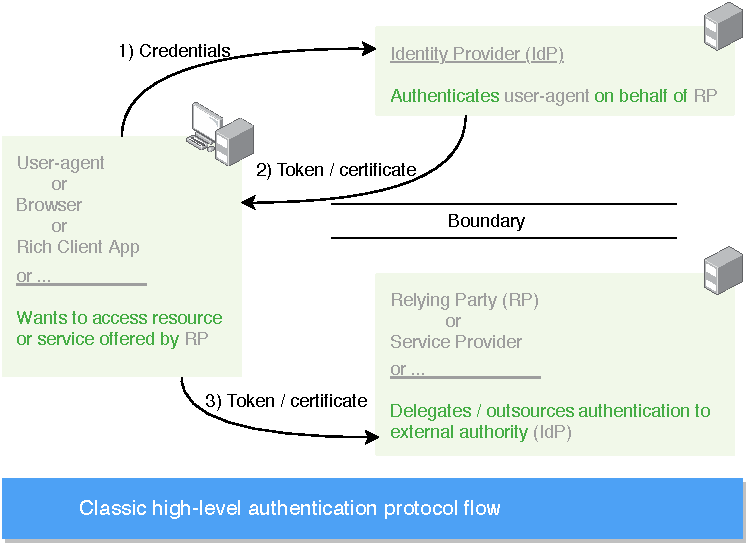
\includegraphics[width=\linewidth]{images/signIn.pdf}
        \caption{Classic high-level authentication protocol flow}
        \label{fig:signin}
    \end{figure}

    %auth delegation problems and necessity,
    Authentication delegation mechanisms are necessary since in all complex systems, we cannot ask every players that provide
    access to services or resources to deal with the management of identities and authentication as well.

    Additionally, while it is true that in theory DAGA can be used anywhere as an ideal replacement of linkable
    ring signatures (LRS) schemes with the added benefit of deniability and forward security\cite{syta_identity_2015},
    the replacement is not straightforward in practise.
    In the LRS case everyone can verify the signature whereas in vanilla DAGA only the cothority is convinced
    of the user authentication\sidenote{and only at the time of verification if there are no other session mechanisms in the picture}
    and the result of the process is only a linkage tag / pseudonymousID that is to be considered public since all the servers
    have access to it.

    The only remaining option, as hinted, would be to require that services interested into using DAGA as authentication mechanism
    be part of the DAGA cothority.
    Not only this is not practical for complex systems, but we would need to either modify the current DAGA cothority code
    to accommodate for such scenarios (e.g.\ provide hooks etc.) or tolerate having specialized version of DAGA nodes for each application.
    Finally this would imply that we are mostly done since the remaining work would be to implement such tight integration mechanisms,
    which is meaningless without having well defined specifications for the services requirements.

    Hence if we want to be as generic and simple as possible and not restrict ourselves with such specific design,
    we need to think of ways allowing to delegate authentication, i.e.\ ways allowing the user-agent to authenticate to the 3rd-party
    with the help of the DAGA cothority.

    \smalltitle{Strawman designs, options}
    To visually represent what has been said above and develop further the options facing us, we start from the following situation:
    \begin{figure}
        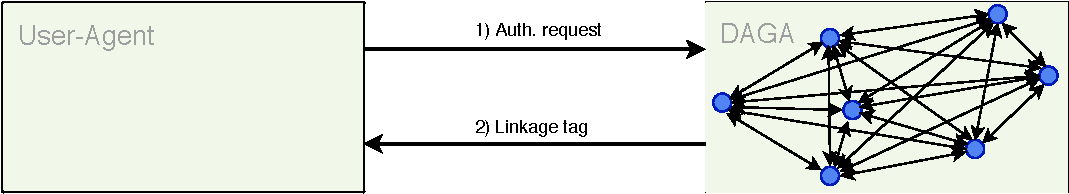
\includegraphics[width=\linewidth]{images/login0_daga.pdf}
        \caption{basic no delegation scenario}
        \label{fig:login0}
    \end{figure}

    As a first way to address the problem mentioned above, we can do the following (for instance):
    \begin{figure}
        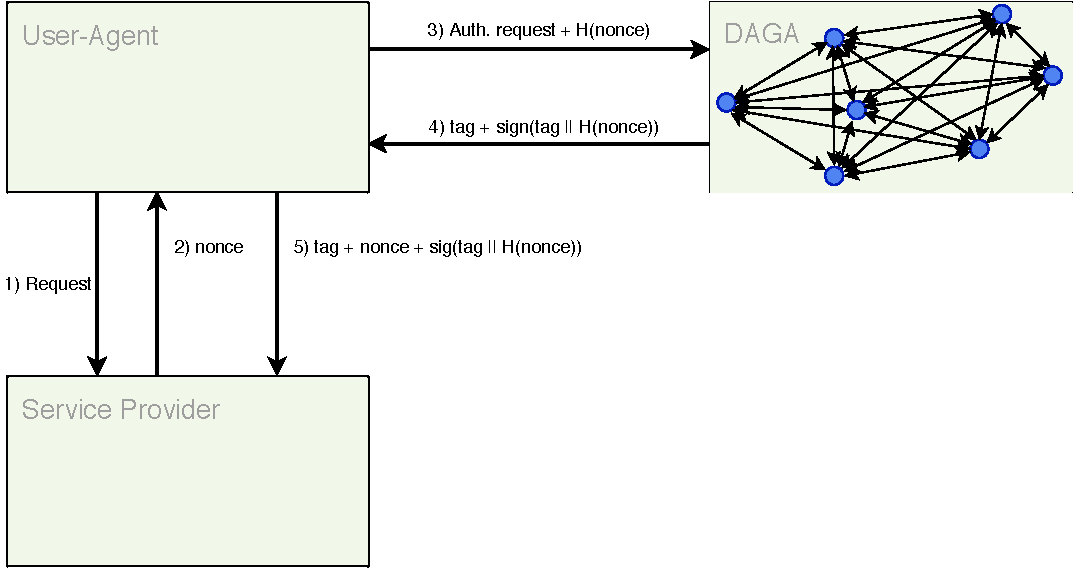
\includegraphics[width=\linewidth]{images/login1_daga.pdf}
        \caption{adds a way to convince 3rd-party that user-agent authenticated with the DAGA cothority}
        \label{fig:login1}
    \end{figure} % TODO modify fig, add explanation for signature in picture, + verification

    But now we just modified the DAGA cothority to make it handle nonces and conversely this requires to closely tie the 3rd-party services
    sign-in code to the DAGA case.
    Another hidden assumption here is that the 3rd-party service has access to the user assets, effectively we put it in a position
    where it can authenticate itself as the user-agent to any authorization mechanism pipelined behind.
    Hence we just restricted ourselves to specific use cases s.t.\ forums or wikis.\newpage

    To address the mentioned issues, we can do the following:
    \begin{figure}
        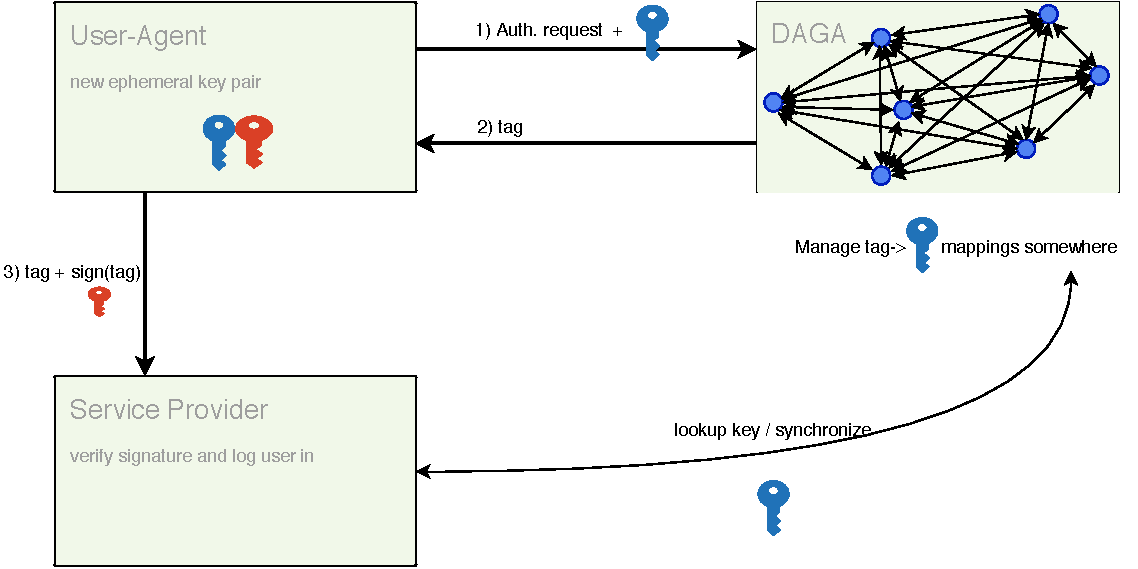
\includegraphics[width=\linewidth]{images/login2_daga.pdf}
        \caption{adds a better way to convince 3rd-party that user-agent authenticated with the DAGA cothority}
        \label{fig:login2}
    \end{figure}

    This is essentially what was described in~\cite[Sect.4.5.1]{syta_identity_2015} and what was done by the dagas
    implementation\sidecite{wolinsy_daga_2014}.
    With each successful authentication the user-agent has the opportunity to register with the cothority a new ephemeral public key
    that is not tied to its long-term ID / public key but to its linkage tag / pseudonymousID\@.
    Furthermore, now the service provider doesn't know the ephemeral secret key and thus cannot authenticate itself as the user-agent.
    \newline
    This is already better than the previous designs since now the cothority is almost not modified, we only need to introduce an additional
    "key server" role that can be implemented in different non-intrusive ways to the cothority implementation\sidenote{
        (e.g. cothority can just publish \(tag \mapsto key\) mappings on a public key-value store etc.)
    }.
    \newline
    However as a new downside we just lost forward-security and deniability, if client's ephemeral secret key is ever compromised we can retroactively
    compromise its anonymity in all past exchanges, since we are now convinced that only it could have issued these signatures.
    In fact looks like we just transformed DAGA into a LRS scheme offering the possibility to rotate keys as a bonus.
    To mitigate this issue we can use very short lived keys etc..
    Additionally we would need to make sure too that any conode processing the request cannot replace the key
    with one under its control.\medskip

    %obvious, interesting but ..offtopic
    %Using the same idea we could even transform the DAGA cothority into a "Deniable Anonymous Group Database" where instead of
    %registering keys the group member can manage some data etc..

    Up to now, all the described approaches are still somewhat home-cooked and not readily interoperable with existing systems
    deployed in production.
    If we want to go down that path and still interface easily with existing systems we would need to provide bridges or
    connectors, one of such option is to provide authentication strategies for well established authentication middleware.
    e.g.\ passport.js, accounts-ui or omniauth for respectively the node.js Meteor and Rails web app worlds.\medskip

    The next and last high-level option we will describe essentially just looks like Fig.~\ref{fig:signin} (see in margin) that introduced
    authentication delegation.
    \begin{marginfigure}
        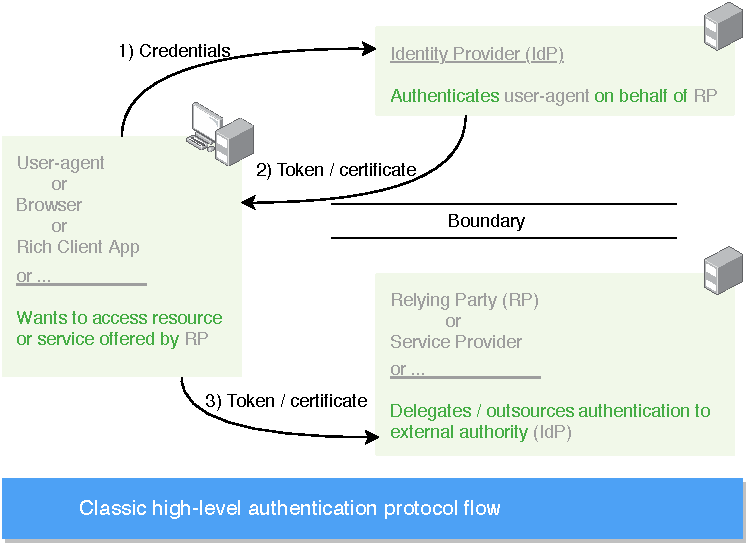
\includegraphics[width=\linewidth]{images/signIn.pdf}
    \end{marginfigure}
    \begin{figure}
        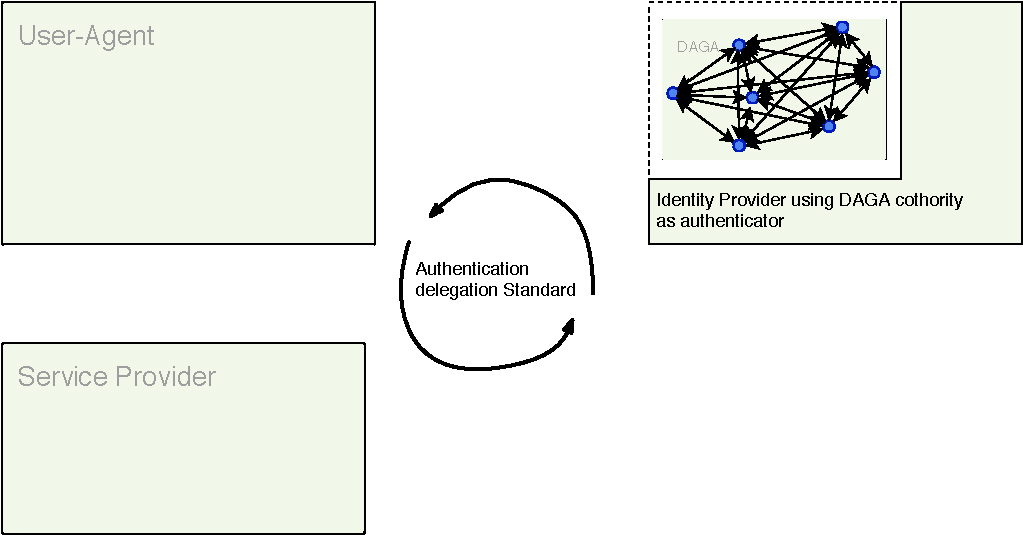
\includegraphics[width=\linewidth]{images/login3_daga.pdf}
        \caption{introduce new trustee entity (IdP) and uses standardized ways to convince 3rd-party that user-agent authenticated with the DAGA cothority}
        \label{fig:login3}
    \end{figure}
    In Fig.~\ref{fig:login3}, instead of reinventing the wheel we rely on existing and well proven protocols and standards for authentication delegation.
    It is the easiest way to have something working quickly and correctly\sidenote{
        designed with care and over time by people and industries that are experts in the field.
        % And thus a design rushed in 2-3 weeks as part of an unrealistic academic project with laughable deadlines cannot compete
    } that would offer us the additional benefit to interface easily with existing services that most definitely already use those mechanisms
    in their authentication workflow.
    To do so we need to introduce a new actor in the picture, the IdP that will use the DAGA cothority as authentication primitive.

    \subsubsection{Chosen solution and PoC}
    Now that we discussed the importance to use an authentication delegation system and exposed different options,
    we need to choose how to implement such system and how it will be used in our PoC\@.
    From the decision keys introduced in the previous description, we chose to use the last option, and we fixed the
    authentication delegation protocol to be OpenID connect.

%    \smalltitle{Background}
    OpenID Connect\sidecite{coreos_openid_nodate} (OIDC) adds an identity layer to, and build upon, the well known OAuth 2.0 authorization framework.
    It is one of the major standard for authentication in the modern world.
    The other choices of framework could have been \emph{SAML}\sidenote{
        Security Assertion Markup Language
    } or eventually Kerberos in controlled environments.

    To build our IdP we chose to use the free-software dex OIDC identity provider which is written in Go and maintained by the CoreOS project.

    Fig.~\ref{fig:poc} describes the system we designed to power the PoC.\
    \begin{figure*}
        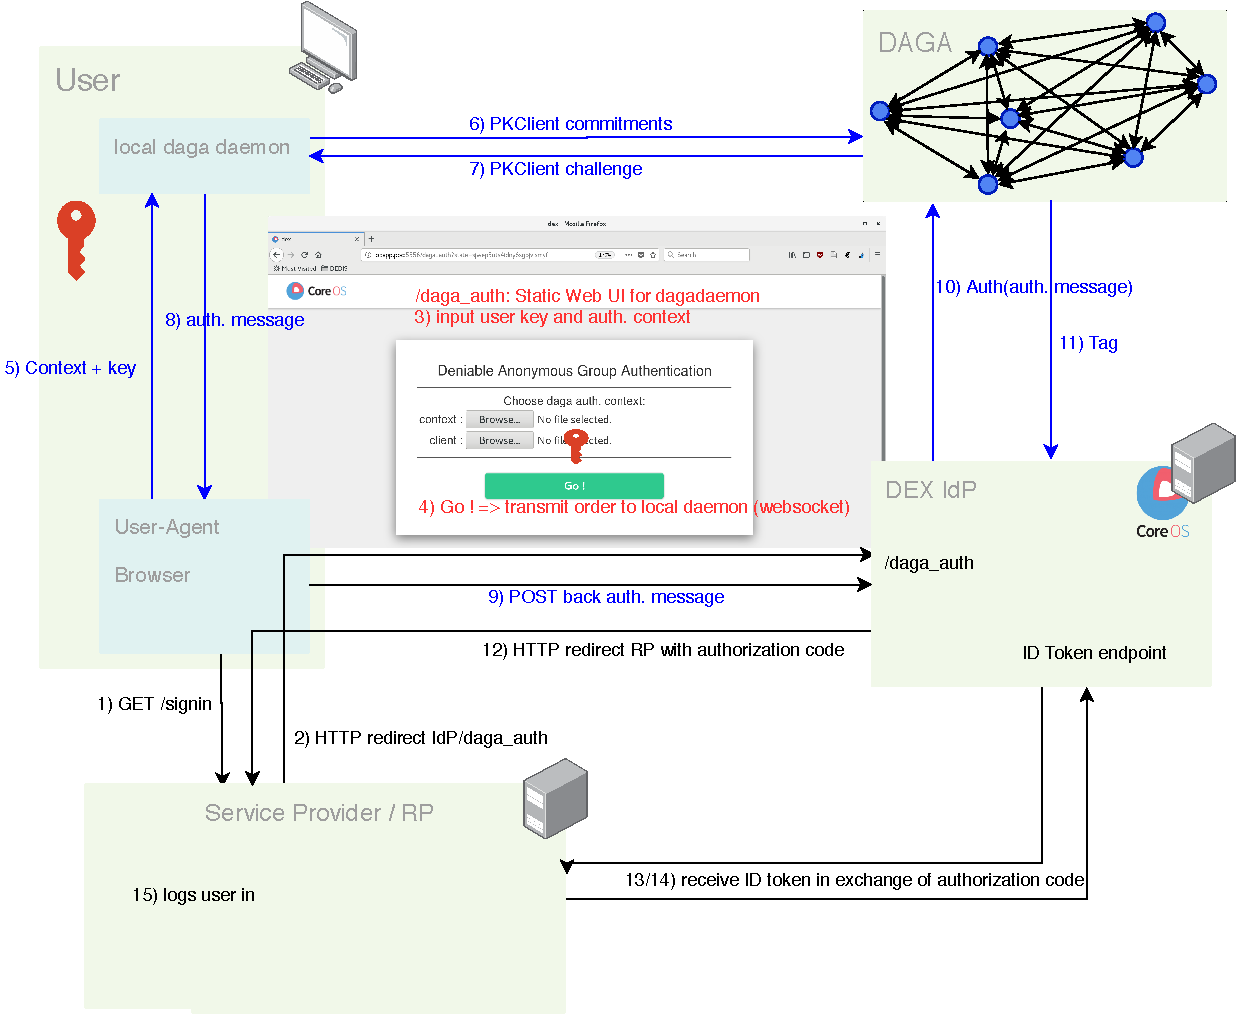
\includegraphics[width=\linewidth]{images/poc.pdf}
        \caption{The designed auth.\ delegation system, the figure shows the standard OIDC code flow as well as the moves related to the
                    DAGA authentication protocol}
        \label{fig:poc}
    \end{figure*}

    The moves in blue are related to the DAGA authentication protocol, the moves in red depicts user input/action and the remaining
    moves in black are the move of the standard OIDC code flow,\sidenote{
        we can choose whichever OIDC flow we want, this is offered for free by OIDC and DEX.
    } where \begin{enumerate}
                \item the RP redirects the user to the IdP
                \item the IdP authenticates the user (here using DAGA)
                \item the IdP redirects back the user to the RP with an authorization code
                \item the RP talks to the IdP to  exchange the authorization code against an ID token which asserts the identity of the user
                \item the RP validates the token and logs the user in
    \end{enumerate}

    The service provider is a dummy express.js app that uses passport.js and an OIDC strategy as its auth.\ middleware to talk to the IdP.\@
    To authenticate the user, the IdP serves a static page that allow the user to select in a graphical and user-friendly way
    the authentication context and its secret identity (index in context + key).
    Then by clicking on the "Go" button, the selected input is forwarded via websocket to a local DAGA daemon\sidenote{
        As we can see in the picture, at no point the private key leave the system of the user.
    } whose role is to conduct the proof of knowledge with the DAGA cothority and to assemble the authentication message.\sidenote{
        This mechanism was introduced mostly for convenience, to avoid having to port the entire DAGA library and client to JS code.
    }
    Once done the message is fed into the websocket channel back to the browser that will upon reception POST it back to the IdP.\
    The IdP will proxy the request to the DAGA cothority and receive the final linkage tag in return.

%    mention undesirable (point of view) side effects of the server proofs
%    (ok can argue that server's proofs (verifiable by anyone)+ anytrust + current description of protocol, sufficient to convince others that auth was done,
%    and to transfer it..was not seen at first)
%    => BUT hehe this means that we weaken deniability (the NIZK proofs of the servers + anytrust ==> someone authenticated for sure)
%    => in fact even in vanilla daga description if we don't publish the server proofs, at the end of successful auth ALL servers obtain all the proofs and tag
%    => since we are in anytrust mean all but one server can be malicious/dishonnest => deniability doesn't hold as advertised in paper (but still)
%    this fact was not seen at first and since time is short (again..)
%    and already decided to not rewrite server part of lib + would need more time
%    to think about it and to see if daga description can be fixed easily without destroying other things,
%    was not done !

    There were other competing alternatives that are worth mentioning and that were kept in case of trouble implementing the OIDC solution.
    \begin{itemize}
        \item design from scratch our IdP as a kind of certificate authority issuing short lived JWT or x.509 certificates for the users.
                and have the users authenticate to the 3rd-party service through HTTP header (JWT) or TLS client-side authentication (x.509).\sidenote{
                    we can note too that there exists readily available passport.js strategies to authenticate users via these certificates.
                }
                To build such CA we even considered using other cothority projects such as ftcosi to make it fully decentralized.
        \item finally in last resort fallback to a custom protocol and offer a passport.js module to interface with it.
                (seems as difficult to learn and implement, if not more (need to modify cothority too), than the other options and restrict the set of users to node.js apps)
    \end{itemize}



    %TODO small conclusion + ref with future/conclusion
    % word on evolution of subscribers/contexts + tracking of # of auth etc.. that is currently not supported
    % Finally the last missing piece to allow all kind of services is ..... currently easyest way would be to revoke and recreate but not practical

%    scratch pad:
%    3) Login service,
%    -don't forget to state/formalize vision of current architecture (actors, roles etc.. trust, etc..)
%    -architecture implementee idee et etat (lack of ssl for now)
%
%    -trusteeOP convinced of auth by the mentioned hole in the design and the fact that he act as a proxy/legalMITM
%    -advantage of introducing this trustee can democratize daga every openid blabla
%
%    potential issue how can a user be convinced that the cothority is not toatally under control of 3rd party service
%    => giving false ssense of securtiy  (outside of scope of porject but worht mentioning )
%
%    -in future can think to move its functionality in the cothority !
%    -cothority service not polluted by design choice of login service
%    -openid connect intro, flows, dex





















